\marginpar{
%\vspace{-5in}
\begin{figure}
  \begin{center}
  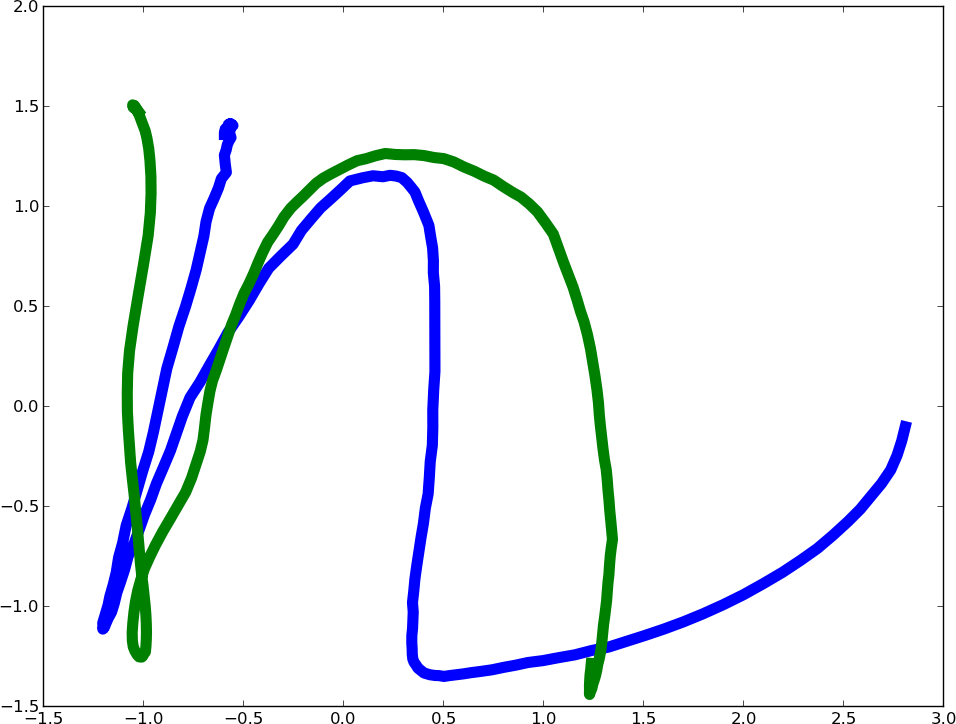
\includegraphics[width=1.5in]{images/new-n-match-cropped.png}
  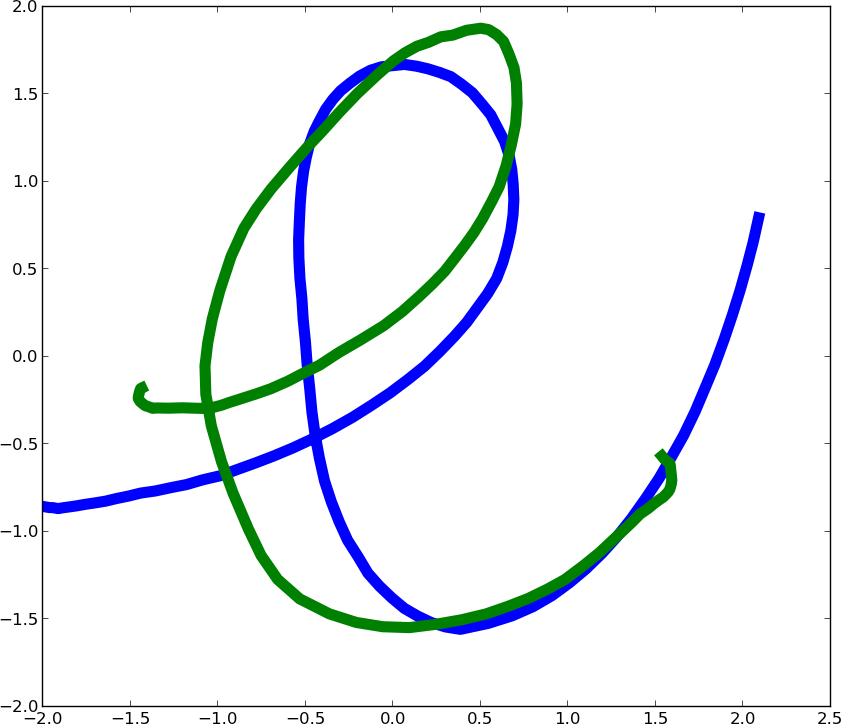
\includegraphics[width=1.5in]{images/new-e-match-cropped.png}
  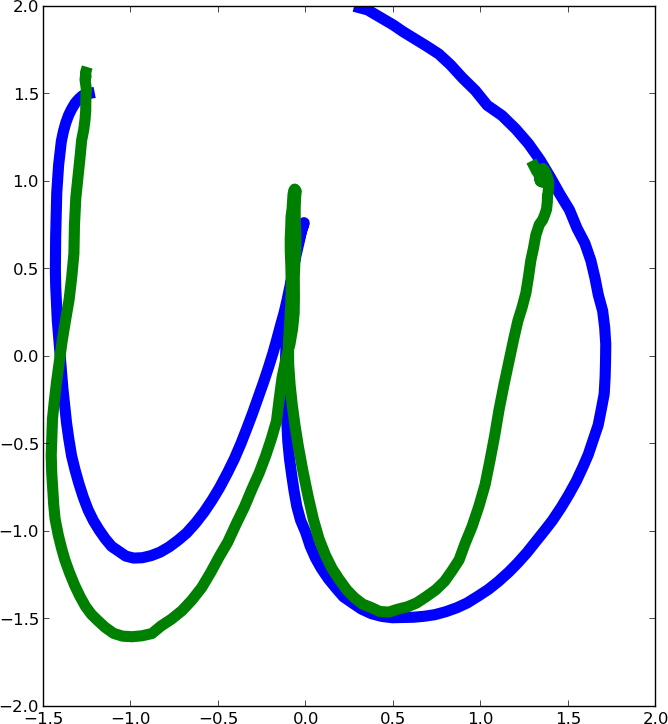
\includegraphics[width=1.5in]{images/new-w-match-cropped.png}
  \caption{The "n", "e", and "w" matches for the "new" time series. Candidates are in green and subsequences from the data are in blue.} 
  \label{fig:n-e-w}
  \end{center}  
\end{figure}
}

Given a set of candidate vectors, a nearest neighbor similarity search across an input time series can be run, searching for the closest subsequence match to the each candidate. Each candidate is a recorded 2D sequence of a letter, which we will call a query and the input finger points will be called the data.
The complexity of the DTW metric is in $O(nr)$ where $n$ is the length of the vectors being compared (or query size) and $r$ is the time window size. A similarity search of a given query vector across a given data vector of length $m$ would be in $O(nrm)$. With a database of query vectors of size $k$, the entire search would be in $O(nrmk)$ time.
Recent optimizations on DTW similarity search can make this entire operation feasible in real time. The optimizations used by this paper are a improved version of the UCR Suite~\cite{rakthanmanon2012searching}, including:
\begin{enumerate*}
\item
Approximated normalization of query and subsequences, and mean and standard deviations are updated rather than recalculated
\item
Cascading the LB Kim and LB Keogh
\item
Using LB Keogh on the subsequence in addition to the query
\item
Sorting the normalized query to abandon earlier when calculating LB Keogh
\end{enumerate*}
A key difference in the proposed method and the UCR Suite is that the UCR Suite was implemented for a univariate time series. Thus, to implement these optimizations, the lower bounding measures had to be extended to a trivariate time series ${x,y,z}$.~\cite{rath2002lower-bounding}
We can also speed up the process by parallelizing the similarity search.
